\newpage
\section{Replication: Synchronizing State}

This section discusses replicating state across distributed systems.

\begin{Def}[Replication]

    \textbf{Replication} is the process of maintaining multiple copies of the same data on different nodes (machines). 
    This is done for fault-tolerance, load balancing, and data locality.
\end{Def}

\noindent
\textbf{Problem Space:}\\
Consider we are running a money transfer service, from which Alice and Bob interact with:
\begin{figure}[h]
    \centering
    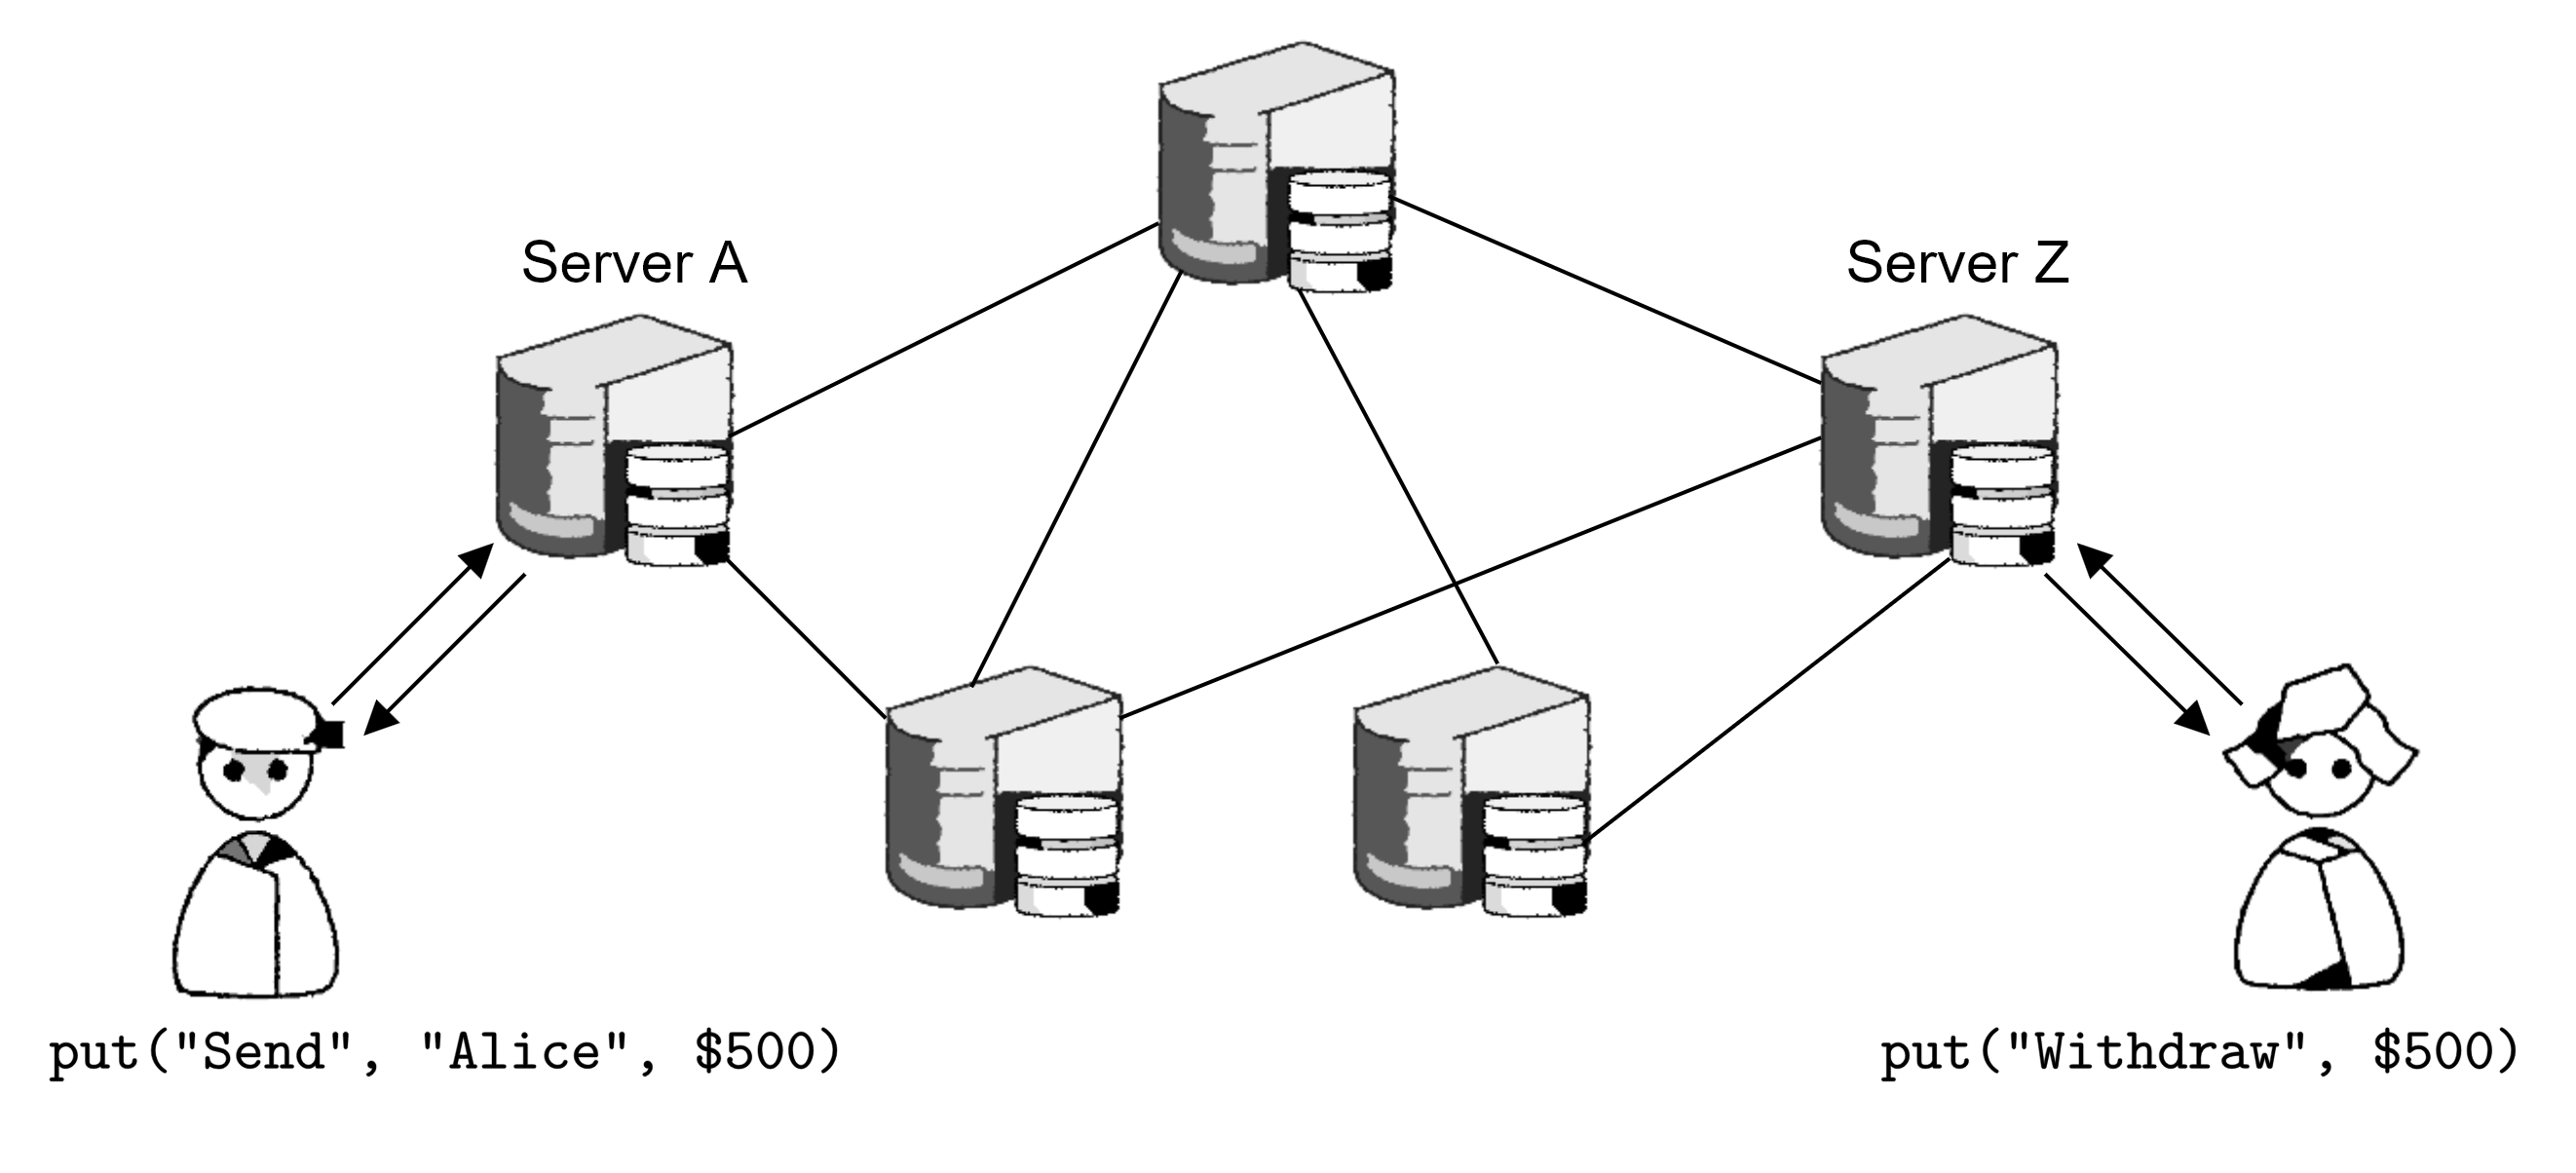
\includegraphics[width=.9\textwidth]{Sections/rep/intro.png}
    \caption{Bob sending money to Alice, while she withdraws money on two different servers.}
\end{figure}

\noindent
In this scenario Many problems can arise: What if,
\begin{itemize}
    \item The respective servers crash while or after Alice or Bob make requests?
    \item Alice and Bob share the same account, how do we ensure consistency?
\end{itemize}

\noindent
In all, wow do we ensure the propagation and synchronization of state across multiple servers?
We consider two models:
\begin{Def}[Active vs. Passive Replication]

    \textbf{Active Replication}: Client sends requests to all servers at the same time and waits for acknowledgments. This method must ensure that all 
    requests are processed in the same order (expensive).\\
    
    \noindent
    \textbf{Passive Replication}: Client sends requests to a primary server, which then forwards the request to backup servers.
\end{Def}

\newpage 

\noindent
We'll be move forward with \textbf{Passive Replication} as the preferred choice in this section.
Though it is less expensive than active replication, it still has its challenges:
\begin{itemize}
    \item \textbf{Consistency}: How do we ensure all backups are consistent?
    \item \textbf{Failure Handling}: What if the primary server fails?
    \item \textbf{Performance}: How do we ensure that the system is performant as we scale backups?
\end{itemize}

\noindent
We consider two methods of replication:
\begin{Def}[State vs. Request Replication]

    \textbf{State Replication}: Forward the entire state to backups. This results in large message sizes, but is relatively simple depending on the system.\\

    \noindent 
    \textbf{Request Replication}: Forward only requests to backups. This results in smaller message sizes, but adds complexity when requests are not deterministic (e.g., random number generation).
\end{Def}

\noindent
Still again, we run into the following problem:
\begin{figure}[h]
    \centering
    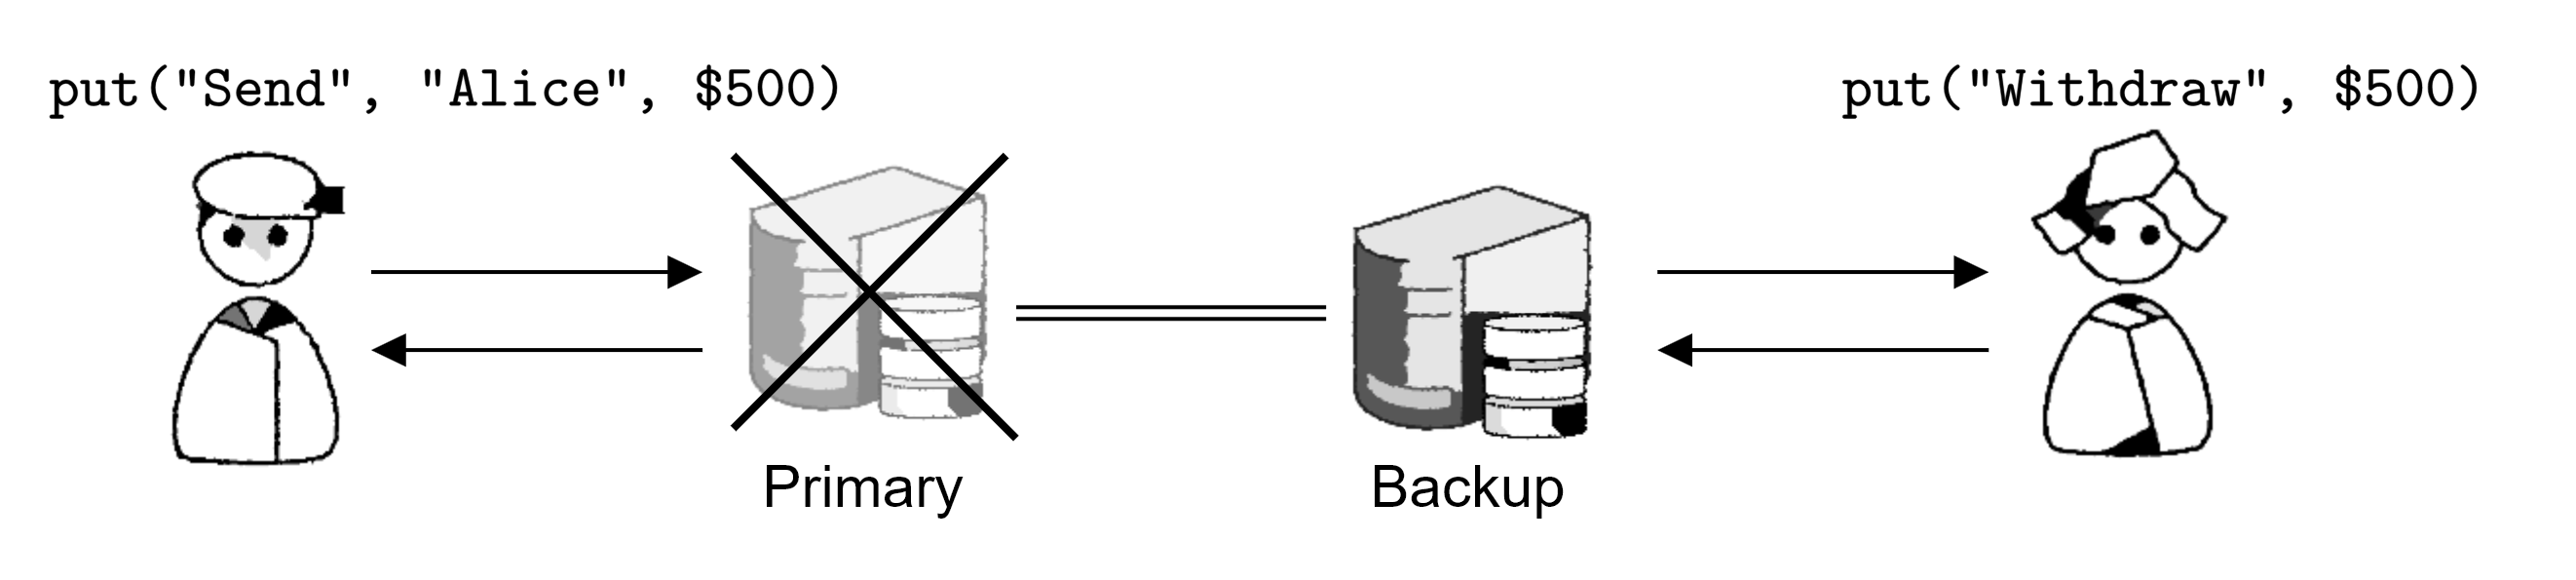
\includegraphics[width=.9\textwidth]{Sections/rep/primary.png}
    \caption{Bob's primary server failing, as Alice accesses the backup server.}
\end{figure}

\noindent
How do we ensure both parties receive consistent feedback, even when the primary server fails?
\begin{Def}[Commit Point]

    The point at which the client is committed to a transaction, goes as follows:
    \begin{enumerate}
        \item The client sends a request to the primary server and waits for an acknowledgment.
        \item The primary server forwards the request to the backup servers.
        \item The backup servers process the request and send an acknowledgment to the primary server.
        \item The primary server sends an acknowledgment to the client.
    \end{enumerate}

    \noindent
    Step 4 is considered the \textbf{commit point}.
\end{Def}

\newpage 

\noindent
The following Figure illustrates the commit point in action:
\begin{figure}[h]
    \centering
    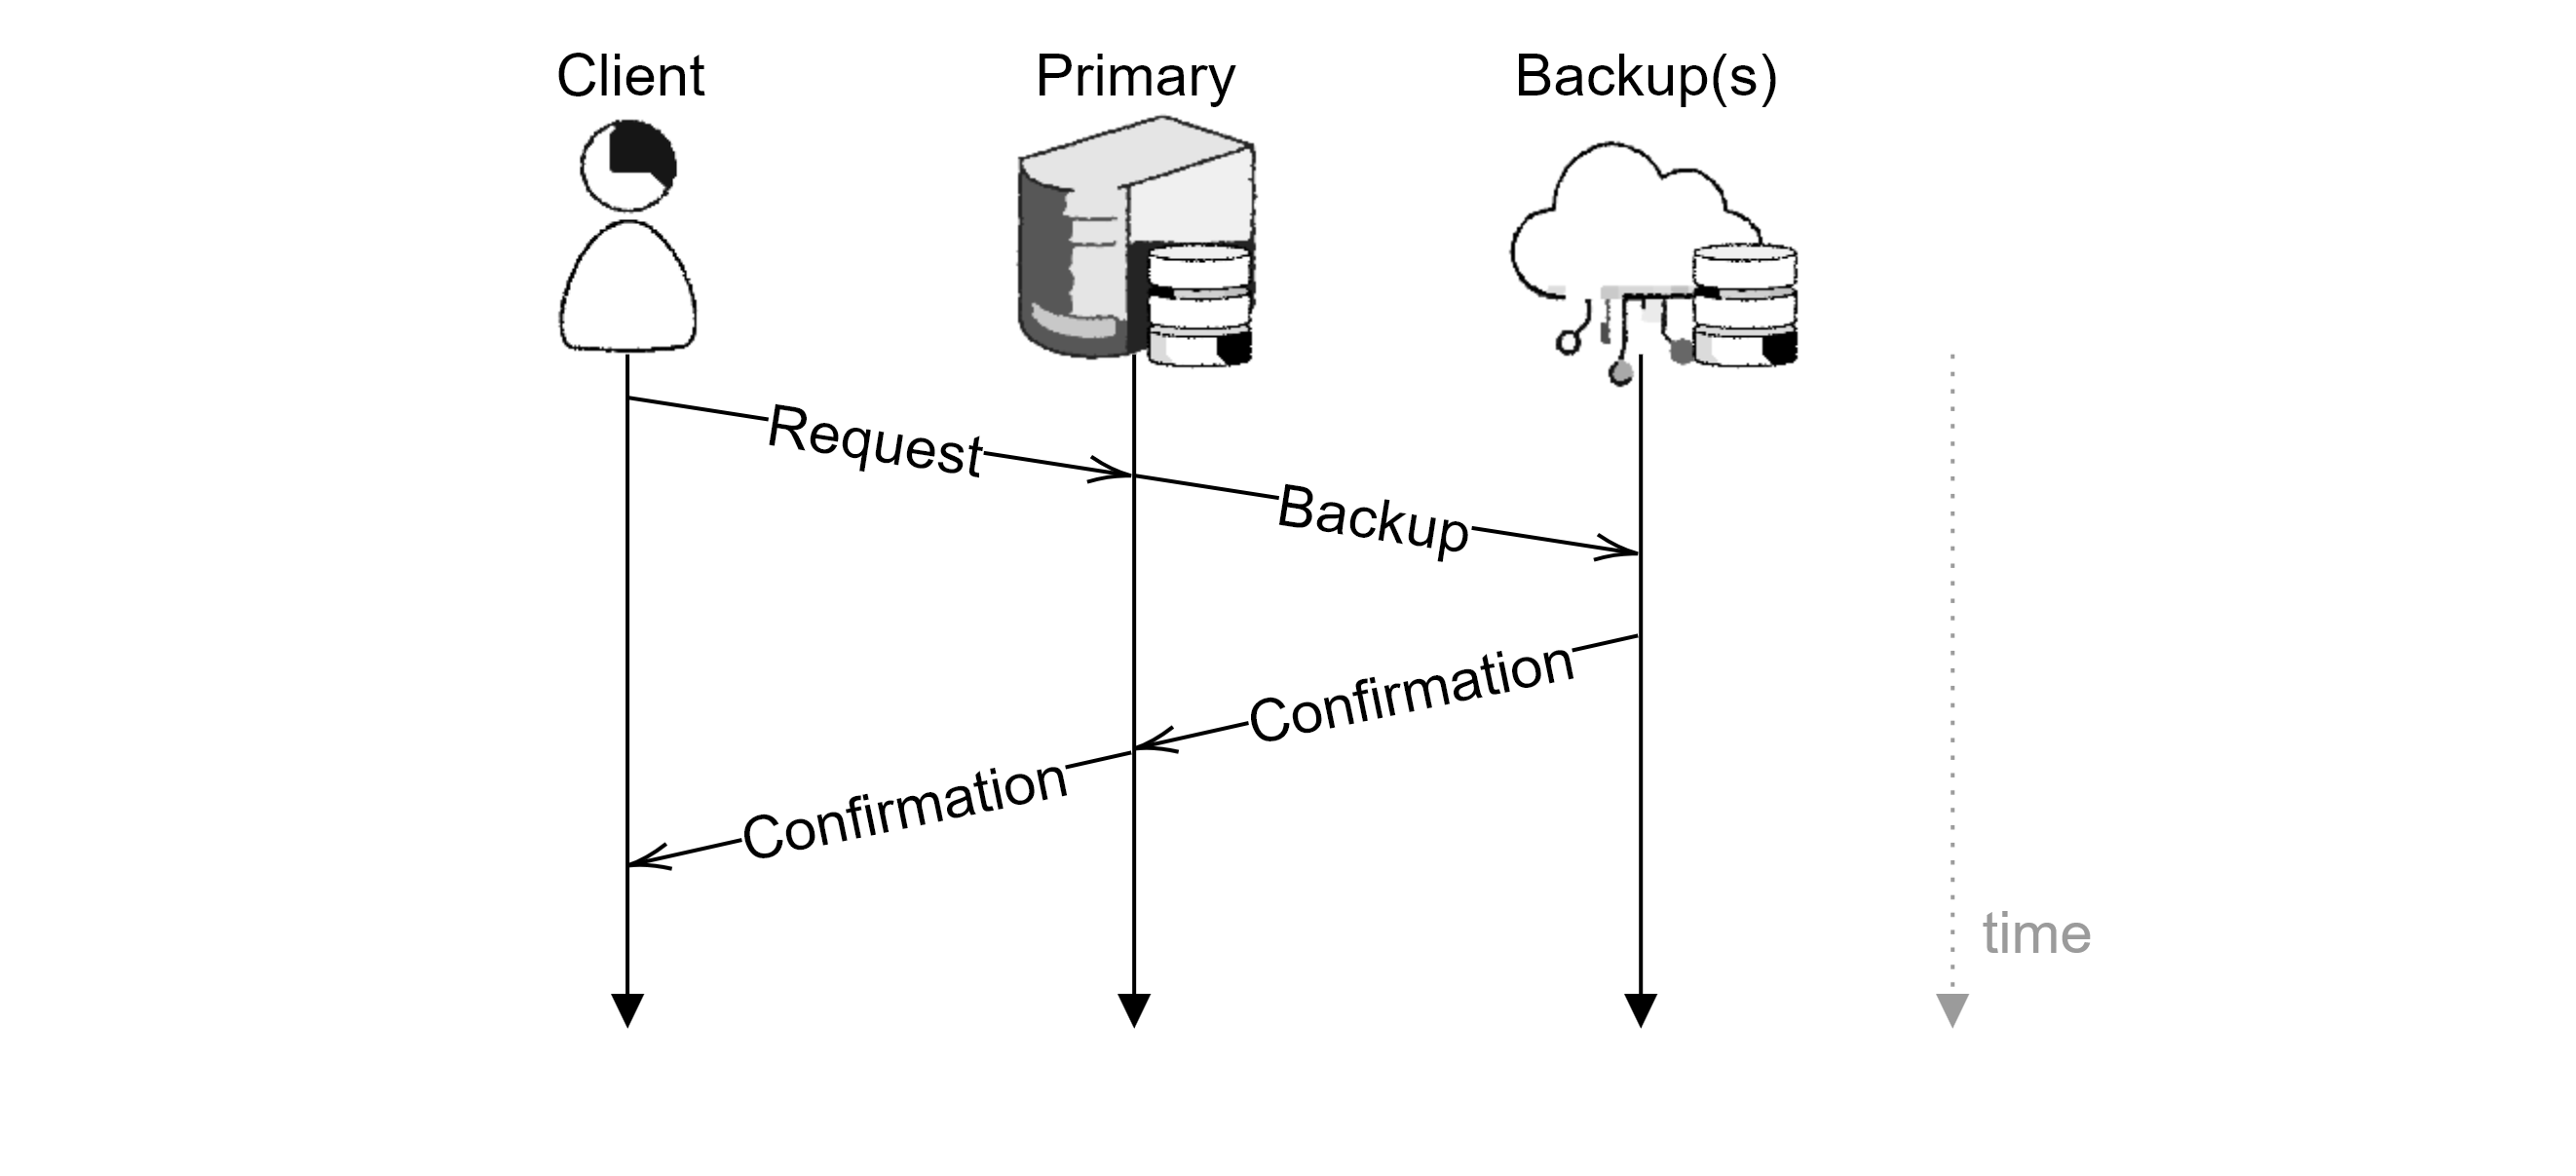
\includegraphics[width=1\textwidth]{Sections/rep/commit.png}
    \caption{Client's requests propagating through the primary and backup sever.}
\end{figure}
